% CS229 Project Milestone --- adapted from /Users/williamtan/Downloads/cs229-milestone.tex
\documentclass{article}

\usepackage[preprint]{cs229}
\usepackage[utf8]{inputenc}
\usepackage[T1]{fontenc}
\usepackage{hyperref}
\usepackage{url}
\usepackage{booktabs}
\usepackage{amsfonts}
\usepackage{nicefrac}
\usepackage{microtype}
\usepackage{xcolor}
\usepackage{amsmath}
\usepackage{fancyhdr}
\usepackage{graphicx}
\usepackage{caption}
\usepackage{subcaption}

\pagestyle{fancy}
\fancyhf{}
\fancyhead[C]{CS229 Project Milestone}
\renewcommand{\headrulewidth}{0.4pt}

\renewcommand{\maketitle}{
  \begin{center}
    \vspace{0.1cm}
    {\bf \large EEG-to-Motion: Decoding Continuous Hand Kinematics\\from Brain Signals with Few-Shot Personalization}\\
    {\bf Team Members:} William Tan, William Wang, Eid Al Aktaa\\
    \vspace{0.1cm}
    {\bf Emails:} willtan@stanford.edu, wwang25@stanford.edu, maktaa@stanford.edu
    \vspace{0.2cm}
  \end{center}
}

\graphicspath{{results/figures/}}

\begin{document}

\maketitle

\section{Motivation}

Brain--computer interfaces (BCIs) promise to restore motor function for individuals with paralysis and to enable natural human--computer interaction without physical input devices. Implantable BCIs (BrainGate, Neuralink, Synchron) have demonstrated clinically meaningful continuous limb control, but only on the order of 80 patients have been implanted worldwide cumulatively, with surgical risk and limited electrode lifetime~\cite{dohle2025}. Non-invasive scalp electroencephalography (EEG) is the only realistic path to mass-scale BCI deployment, but the dominant blocker for deployable EEG BCIs is \emph{per-user calibration cost}: classical decoders require 15--30 minutes of supervised setup before they are operable~\cite{lotte2015}, and patients and consumer users will not tolerate this on every session.

This project asks two questions: (1) can a deep learning model trained on a population of EEG users accurately decode continuous hand kinematics from scalp EEG, and (2) how much per-user calibration data is required, and which adaptation method is most efficient, to bring a new user's performance close to that of a fully personalized model. These quesitons positions our work alongside two recent successful advancements: MindEye2~\cite{mindeye2}, which decodes functional MRI (fMRI)-to-image with $\sim$1 hour of per-subject data on a shared backbone, and Meta sEMG~\cite{metaemg}, which achieves cross-person surface electromyography (sEMG) decoding with \emph{zero} per-user calibration. Continuous motor regression is a documented gap in the foundation-model-for-EEG literature (LaBraM~\cite{labram}, CBraMod~\cite{cbramod}, EEGPT~\cite{eegpt}, NeuroLM~\cite{neurolm} all evaluate primarily on classification).

We hypothesize that continuous hand-kinematic decoding from scalp EEG is bottlenecked not by raw decoder capacity but by per-user calibration cost. Foundation-model pretraining on cross-subject corpora, combined with calibration-efficient adaptation, can drive new-user calibration from the field-standard 20--30 minutes to the single-digit-minute regime while preserving most of within-subject performance, but only when evaluated under strict artifact and causal-filter controls~\cite{antelis2013}.

\section{Methods}

\paragraph{Dataset.} Our preliminary experiments use \textbf{WAY-EEG-GAL}~\cite{way-eeg-gal}, which provides 12 healthy participants performing instrumented grasp-and-lift trials of an object whose weight (165/330/660\,g) and surface (sandpaper/suede/silk) vary unpredictably. Each subject has 9 series of $\sim$32 trials with 32-channel scalp EEG sampled at 500\,Hz, Polhemus FASTRAK electromagnetic tracker capturing 3D hand position at 500\,Hz, plus 5-channel surface electromyography (EMG) and 6-axis force/torque on the contact plates. We use subjects P1, P2, and P3 across all 9 series ($\sim$30 minutes of recorded EEG per subject, 294 trials each). Preprocessing applies common-average referencing, a fourth-order zero-phase Butterworth band-pass at 0.1--40\,Hz, downsampling 500$\to$100\,Hz, and per-channel trial-wise z-scoring. Kinematic targets are 3D hand velocity (mm/s), obtained by low-passing position at 5\,Hz, downsampling to match the EEG grid, and differentiating. We chose velocity over position to align with the Bradberry 2010~\cite{bradberry2010} / Müller-Putz~\cite{mondini2020} literature and to remove low-frequency position drift confounds. The final project will extend to Jeong 2020 (25 subjects $\times$ 3 sessions one week apart)~\cite{jeong2020} and the Müller-Putz ``Feel Your Reach'' line~\cite{mondini2020} to support cross-session calibration curves with measured 2D end-effector trajectories.

\paragraph{Decoders.} We benchmark four baselines spanning the canonical capacity ladder for EEG decoding: (1) \textbf{Bradberry-mLR} (multivariate linear regression), ridge regression on lag-augmented low-frequency potentials (lags 0--250\,ms), replicating Bradberry~\cite{bradberry2010}; (2) \textbf{Ridge-BandPower}, ridge regression on log-band-power features in $\mu$ (8--13\,Hz), $\beta$ (13--30\,Hz), and low-$\gamma$ (30--45\,Hz) bands within 500\,ms sliding windows, in the Korik~\cite{korik2018} ``band-time-series'' style; (3) \textbf{EEGNet}~\cite{eegnet} ($\sim$3k parameters) with a 3-output linear regression head; and (4) \textbf{ShallowConvNet}~\cite{shallowconv} ($\sim$50k parameters) with a 3-output linear head, whose log-band-power readout mirrors Filter Bank Common Spatial Patterns (FBCSP). Neural nets train with AdamW, MSE loss, target z-scoring, gradient clipping at norm 1.0, early stopping on a 10\% validation split.

\paragraph{Evaluation framework.} The same framework will be used to evaluate the foundation-model SOTA in the next phase, so its design is deliberate. We report Pearson $r$ per axis and averaged (the field-standard metric kept for comparability with~\cite{bradberry2010,mondini2020,borra2023}) alongside $R^2$, RMSE in mm/s, and a \textbf{circularly-shifted-target permutation null} (200 permutations per fold). The permutation null directly addresses the Antelis 2013~\cite{antelis2013} critique that linear-regression correlations on smooth low-frequency targets can be inflated by ordinary-least-squares (OLS) leakage with no underlying motor information. We also report block-bootstrap 95\% confidence intervals (CIs) and the fraction of subjects exceeding the operational threshold $r > 0.2$. Two evaluation protocols: (W) within-subject 5-fold cross-validation (CV), the personalized-decoder ceiling; and (L) \textbf{leave-one-subject-out (LOSO)} zero-shot transfer, in which we train on $N{-}1$ subjects pooled and evaluate on the held-out target with no target-side data at all. The gap between (W) and (L) is the \emph{personalization gap} the final paper proposes to close.

\section{Preliminary Experiments and Results}

The full grid (3 subjects $\times$ 4 models $\times$ \{5 within-subject folds + 3 LOSO conditions\}) runs in $\sim$28 minutes on a single M-series Mac.

\begin{table}[h]
\centering
\footnotesize
\setlength{\tabcolsep}{4pt}
\begin{tabular}{lrrrrr}
\toprule
Model & Within $r$ & LOSO $r$ & Pers.\ gap & Within $R^2$ & RMSE (mm/s) \\
\midrule
Bradberry-mLR (linear)         & $+0.223 \pm 0.038$ & $+0.091$ & $-59\%$ & $+0.057$ & $1.66$ \\
Ridge-BandPower (linear)       & $+0.127 \pm 0.022$ & $-0.024$ & collapse & $+0.016$ & $1.72$ \\
EEGNet ($\sim$3\,k)            & $+0.176 \pm 0.065$ & $+0.115$ & $-35\%$ & $+0.044$ & $1.66$ \\
ShallowConvNet ($\sim$50\,k)   & $\mathbf{+0.235 \pm 0.044}$ & $\mathbf{+0.130}$ & $-45\%$ & $+0.064$ & $1.61$ \\
\bottomrule
\end{tabular}
\caption{Pearson $r$ averaged across X/Y/Z velocity axes; ``Within $r$'' is mean$\,\pm\,$std across subjects (5-fold CV averaged within each). LOSO = mean across 3 held-out subjects with $N{-}1{=}2$ pooled training subjects. NaN folds excluded via \texttt{nanmean}.}
\label{tab:headline}
\end{table}

\begin{figure}[h]
\centering
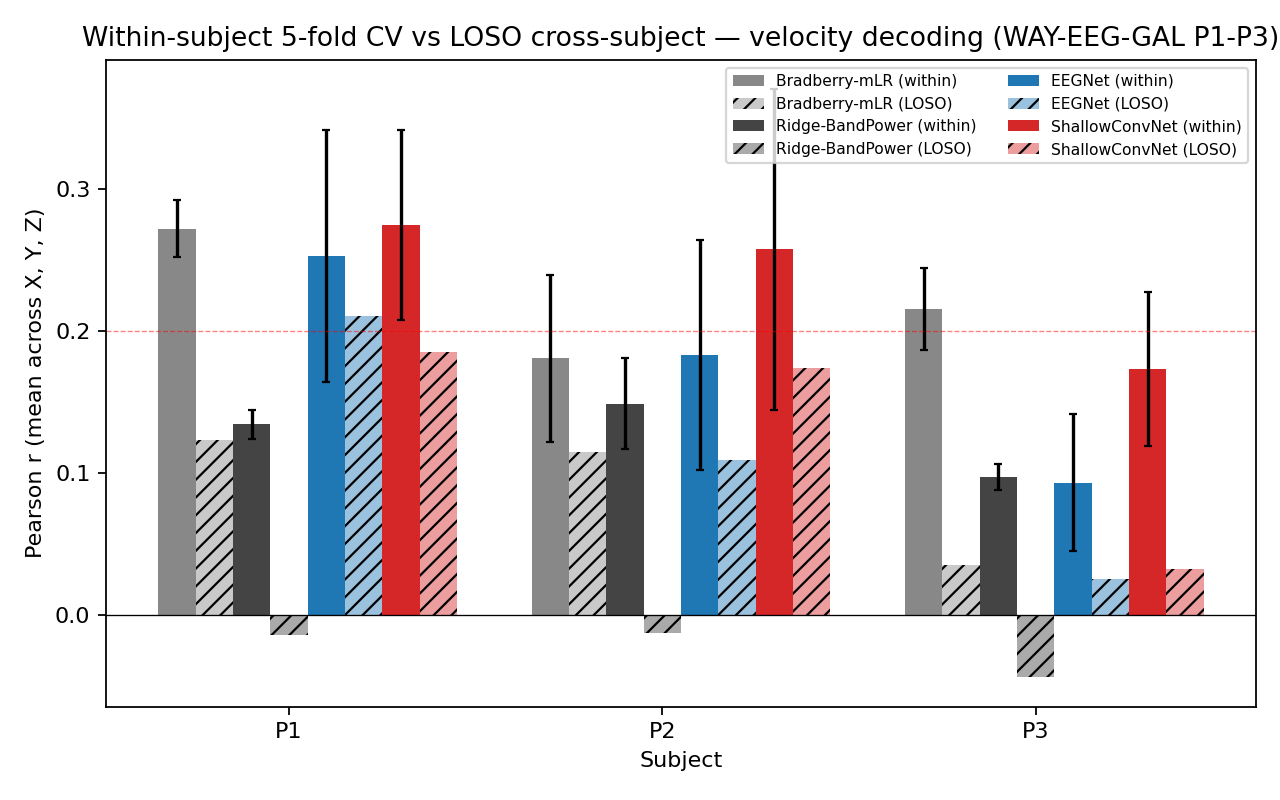
\includegraphics[width=0.92\linewidth]{within_vs_loso_r.png}
\caption{Within-subject 5-fold CV (solid) vs. leave-one-subject-out (hatched). The solid bars are what a fully personalized decoder achieves; the hatched bars are zero-shot transfer with no target-side calibration. The visible gap between solid and hatched is the \emph{personalization gap} the final paper proposes to close with calibration-efficient adaptation. Red dashed line at $r = 0.2$ marks the operational deployment threshold.}
\label{fig:within_vs_loso}
\end{figure}

\paragraph{The signal is real and above the artifact null.} Within-subject Bradberry $r \approx 0.22$ across 3 subjects is squarely in the published range of $0.19$--$0.38$~\cite{bradberry2010}. The Z (vertical lift) axis dominates across every model (Fig.~\ref{fig:per_axis}: ShallowConvNet Z $= 0.41$, EEGNet Z $= 0.34$, Bradberry Z $= 0.33$, Ridge-BP Z $= 0.20$), consistent with the grasp-and-lift physics. More importantly, our permutation null (Fig.~\ref{fig:perm_null}) shows that \textbf{11 of 12 model $\times$ subject combinations clear the $\alpha = 0.05$ null threshold} ($p \leq 0.045$), with the lone failure (EEGNet on P2, $p = 0.158$) coinciding with the lowest-signal subject $\times$ model combination in our data. This is exactly the methodological control the Antelis~\cite{antelis2013} critique demands, and our results survive it.

\begin{figure}[h]
\centering
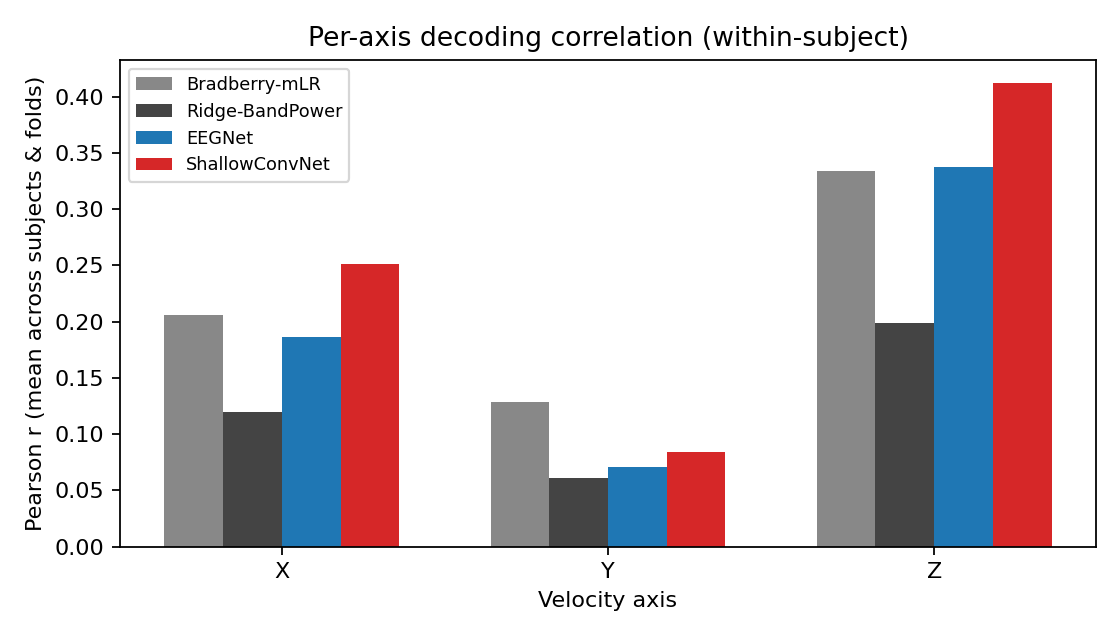
\includegraphics[width=0.62\linewidth]{per_axis_r.png}
\caption{Per-axis Pearson $r$, mean across subjects and folds. Z (vertical lift) dominates across all four models as expected for a grasp-and-lift task; Y (lateral) is the hardest.}
\label{fig:per_axis}
\end{figure}

\begin{figure}[h]
\centering
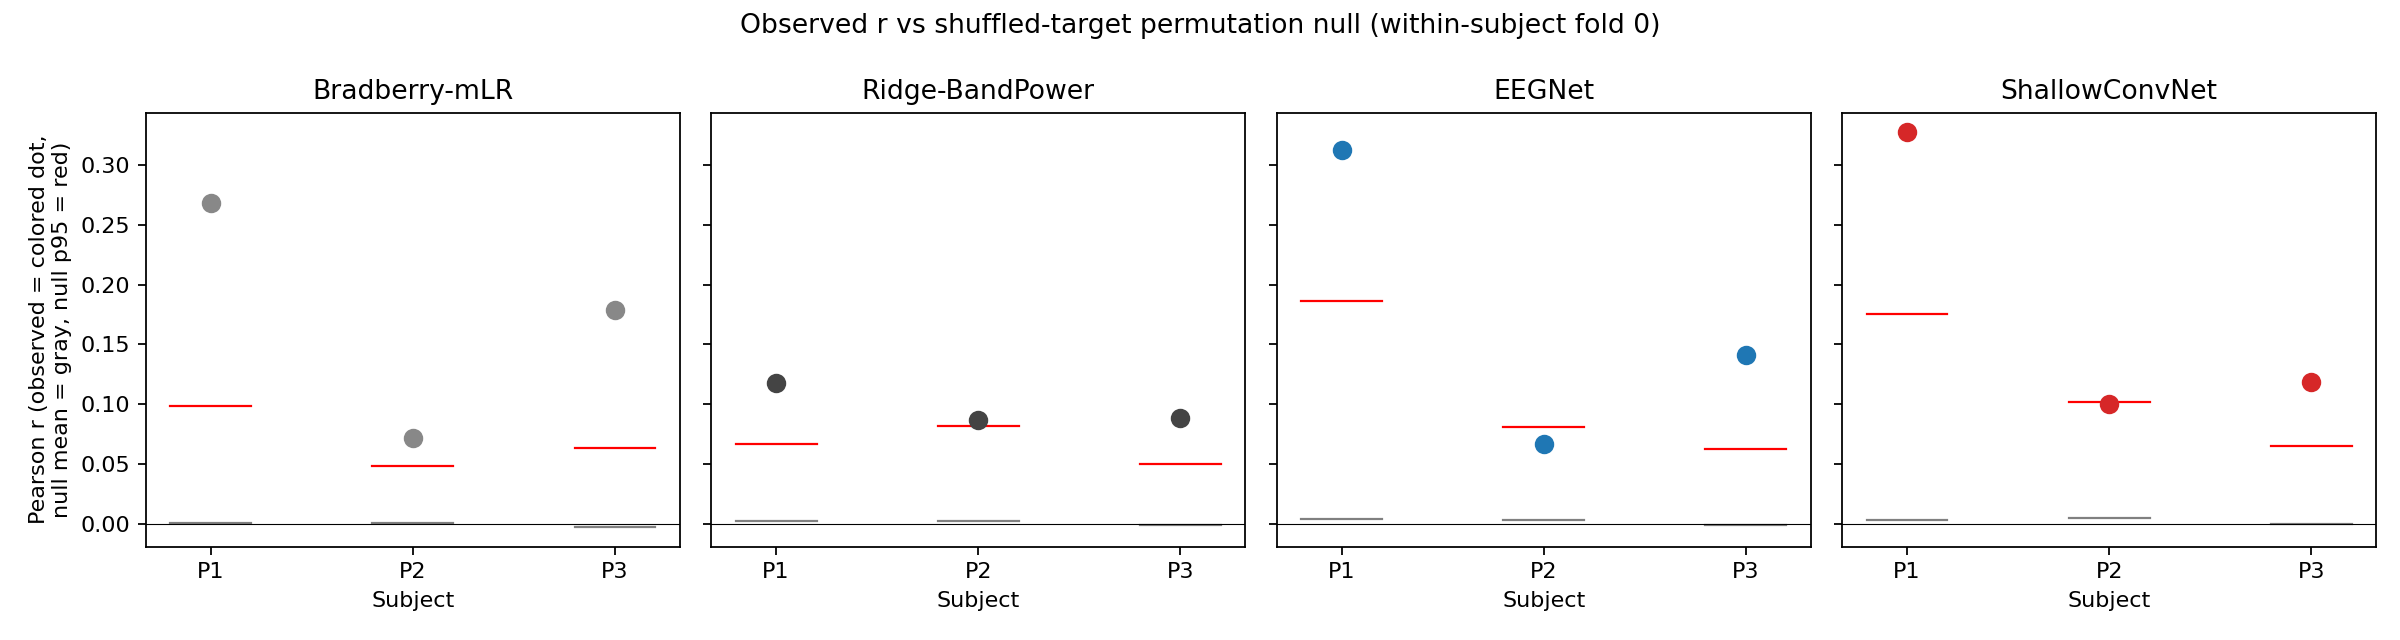
\includegraphics[width=\linewidth]{perm_null.png}
\caption{Observed $r$ (colored dots) vs. shuffled-target permutation null (fold 0 of each within-subject run; 200 permutations each). Gray horizontal line = null mean; red horizontal line = null 95th percentile. Dots above the red line are significant at $\alpha = 0.05$. Result: \textbf{11 of 12} model $\times$ subject combinations clear the null; the lone failure is EEGNet on the lowest-signal subject P2 ($p = 0.158$).}
\label{fig:perm_null}
\end{figure}

\paragraph{The personalization gap is real and large.} All four models lose 35--60\% of their within-subject performance under zero-shot LOSO (Table~\ref{tab:headline}, Figure~\ref{fig:within_vs_loso}). This gap is the central quantity our final paper proposes to close.

\paragraph{The within-subject vs. LOSO ranking inverts.} ShallowConvNet wins both within-subject ($r = 0.235$) and LOSO ($r = 0.130$). But Bradberry-mLR is second within-subject and \emph{fourth} on LOSO showing that its linear features overfit on per-subject electrode patterns. EEGNet shows the \emph{least relative drop} ($-35\%$), suggesting that with more training data, neural features may transfer best. This is our foundation-model thesis: pool more data, train a more flexible model, and cross-subject performance, not within-subject, becomes the headline number.

\paragraph{Inter-subject variability is large even at $N = 3$.} P1's within-subject mean $r$ is $0.272$ (Bradberry); P3's is $0.215$; but P3's LOSO is just $0.04$ across all models. P3 reads as a plausible ``BCI illiteracy''-type subject for this task. The final paper must report per-subject distributions, not just averages and this preliminary finding already justifies that decision.

\paragraph{Neural-net training is unstable on small per-subject data.} EEGNet and ShallowConvNet diverged to NaN (not-a-number, indicating loss explosion or weight overflow) on 9 of 30 within-subject folds (30\%), concentrated in the lowest-signal subject (P3: 6/10 neural-net folds). LOSO with pooled 2-subject data had \emph{zero} NaN failures across 6 neural-net runs. This is itself a finding: at the $\sim$30-minute per-subject scale, the neural-net win over linear baselines is contingent on enough pooled training data.

\section{Next Steps}

\paragraph{Scale up baselines, fix instability.} Extend the preliminary pipeline from 3 to all 12 WAY-EEG-GAL subjects so the per-subject distribution is meaningful, and add the Jeong 2020 dataset~\cite{jeong2020} (25 subjects $\times$ 3 sessions one week apart) as a second corpus to demonstrate cross-corpus generality and unlock the cross-session calibration regime. Fix the NN instability (Huber loss, smaller head init, validation-loss divergence reset) so we no longer drop $\sim$30\% of NN folds to NaN.

\paragraph{Foundation-model backbone and adaptation methods.} Plug in a publicly released EEG foundation model --- EEGPT~\cite{eegpt} (10M params, single-GPU friendly) --- and benchmark linear probe vs.\ full fine-tune against our four classical baselines. Implement three adaptation methods spanning the calibration spectrum: zero-shot LOSO (no target data), Euclidean Alignment~\cite{he2020ea} (zero \emph{labeled} target data), and $K$-minute supervised fine-tune. 

\paragraph{Headline figure and writing.} Produce the \textbf{calibration dose-response curve}: x-axis = per-user calibration budget $K \in \{0, 1, 2, 5, 10, 15, 30~\text{min}\}$; y-axis = Pearson $r$ averaged across held-out subjects with block-bootstrap 95\% CI shading; one curve per adaptation method, with the within-subject ceiling as a horizontal asymptote.

% \paragraph{Honest contingencies.} If Euclidean Alignment recovers most of the gap with zero labeled target data, the calibration story becomes ``you don't need any'' --- still publishable as a useful negative result. If the EEGPT backbone underperforms our linear baselines on regression, the result \emph{is} the contribution: the first published critical evaluation of FM-for-EEG on continuous behavior decoding. The realistic publication target is a workshop paper (NeurIPS Foundation Models for Brain and Body, or ICLR Time Series for Health), not a main-track submission.

\section{Team Contributions}

\begin{itemize}
    \item \textbf{William Tan}: project scaffolding (program all scripts); WAY-EEG-GAL data ingestion and preprocessing pipeline; the four baseline decoders (Bradberry mLR, Ridge BandPower, EEGNet, ShallowConvNet) and runs preliminary within-subject 5-fold CV and leave-one-subject-out experiments.
    \item \textbf{William Wang}: literature review across datasets, architectures, and cross-subject transfer methods; survey of recent top-venue ML papers (NeurIPS/ICLR/ICML 2022--2026) on EEG and biosignal foundation models; methodological-critique reading (Antelis, Whitham, Castermans); thesis framing and motivation drafting.
    \item \textbf{Eid Al Aktaa}: evaluation framework (Pearson $r$, $R^2$, RMSE, shuffled-target permutation null with circular time-shift, block-bootstrap 95\% CIs); statistical analysis of preliminary results; figure generation; drafting of this milestone document.
\end{itemize}

\pagebreak

\begin{thebibliography}{99}

\bibitem[Bradberry et al.(2010)]{bradberry2010}
Bradberry, T. J., Gentili, R. J., \& Contreras-Vidal, J. L. (2010). Reconstructing three-dimensional hand movements from noninvasive electroencephalographic signals. \textit{Journal of Neuroscience}, 30(9), 3432--3437.

\bibitem[Antelis et al.(2013)]{antelis2013}
Antelis, J. M., Montesano, L., Ramos-Murguialday, A., Birbaumer, N., \& Minguez, J. (2013). On the usage of linear regression models to reconstruct limb kinematics from low frequency EEG signals. \textit{PLOS ONE}, 8(4), e61976.

\bibitem[Luciw et al.(2014)]{way-eeg-gal}
Luciw, M. D., Jarocka, E., \& Edin, B. B. (2014). Multi-channel EEG recordings during 3,936 grasp and lift trials with varying weight and friction. \textit{Scientific Data}, 1, 140047.

\bibitem[Mondini et al.(2020)]{mondini2020}
Mondini, V., Kobler, R. J., Sburlea, A. I., \& Müller-Putz, G. R. (2020). Continuous low-frequency EEG decoding of arm movement for closed-loop, natural control of a robotic arm. \textit{Journal of Neural Engineering}, 17(4), 046031.

\bibitem[Jeong et al.(2020)]{jeong2020}
Jeong, J.-H., Cho, J.-H., Shim, K.-H., et al. (2020). Multimodal signal dataset for 11 intuitive movement tasks from single upper extremity during multiple recording sessions. \textit{GigaScience}, 9(10), giaa098.

\bibitem[Korik et al.(2018)]{korik2018}
Korik, A., Sosnik, R., Siddique, N., \& Coyle, D. (2018). Decoding imagined 3D hand movement trajectories from EEG: evidence to support the use of mu, beta, and low gamma oscillations. \textit{Frontiers in Neuroscience}, 12, 130.

\bibitem[Borra et al.(2023)]{borra2023}
Borra, D., Magosso, E., \& Ravanelli, M. (2023). Decoding movement kinematics from EEG using an interpretable convolutional neural network. \textit{Computers in Biology and Medicine}, 165, 107323.

\bibitem[Lawhern et al.(2018)]{eegnet}
Lawhern, V. J., Solon, A. J., Waytowich, N. R., et al. (2018). EEGNet: a compact convolutional neural network for EEG-based brain--computer interfaces. \textit{Journal of Neural Engineering}, 15(5), 056013.

\bibitem[Schirrmeister et al.(2017)]{shallowconv}
Schirrmeister, R. T., Springenberg, J. T., Fiederer, L. D. J., et al. (2017). Deep learning with convolutional neural networks for EEG decoding and visualization. \textit{Human Brain Mapping}, 38(11), 5391--5420.

\bibitem[Jiang et al.(2024)]{labram}
Jiang, W.-B., Zhao, L.-M., \& Lu, B.-L. (2024). Large Brain Model for learning generic representations with tremendous EEG data in BCI. \textit{ICLR 2024} (spotlight).

\bibitem[Wang et al.(2025)]{cbramod}
Wang, J., et al. (2025). CBraMod: a criss-cross brain foundation model for EEG decoding. \textit{ICLR 2025}.

\bibitem[Wang et al.(2024)]{eegpt}
Wang, G., et al. (2024). EEGPT: pretrained transformer for universal and reliable representation of EEG signals. \textit{NeurIPS 2024}.

\bibitem[Jiang et al.(2025)]{neurolm}
Jiang, W.-B., et al. (2025). NeuroLM: a universal multi-task foundation model for bridging the gap between language and EEG signals. \textit{ICLR 2025}.

\bibitem[Scotti et al.(2024)]{mindeye2}
Scotti, P. S., Tripathy, M., Torrico-Villanueva, C., et al. (2024). MindEye2: shared-subject models enable fMRI-to-image with 1 hour of data. \textit{ICML 2024}.

\bibitem[Sivakumar et al.(2025)]{metaemg}
Sivakumar, A. R., et al. (2025). A generic non-invasive neuromotor interface for human--computer interaction. \textit{Nature}, 645, 1--10.

\bibitem[He \& Wu(2020)]{he2020ea}
He, H., \& Wu, D. (2020). Transfer learning for brain--computer interfaces: a Euclidean space data alignment approach. \textit{IEEE Transactions on Biomedical Engineering}, 67(2), 399--410.

\bibitem[Mellot et al.(2024)]{gopsa2024}
Mellot, A., Collas, A., Gramfort, A., \& Engemann, D. (2024). Geodesic optimization for predictive shift adaptation on EEG data. \textit{NeurIPS 2024}.

\bibitem[Vidaurre \& Blankertz(2010)]{vidaurre2010}
Vidaurre, C., \& Blankertz, B. (2010). Towards a cure for BCI illiteracy. \textit{Brain Topography}, 23(2), 194--198.

\bibitem[Lotte(2015)]{lotte2015}
Lotte, F. (2015). Signal processing approaches to minimize or suppress calibration time in oscillatory activity-based brain--computer interfaces. \textit{Proceedings of the IEEE}, 103(6), 871--890.

\bibitem[Dohle et al.(2025)]{dohle2025}
Dohle, J., et al. (2025). Implantable brain--computer interfaces for motor impairment: a systematic review. \textit{Advanced Science}, 12, 2501912.

\end{thebibliography}

\end{document}
